\documentclass[aspectratio=169]{beamer}
\mode<presentation>
%\usetheme{Warsaw}
%\usetheme{Goettingen}
\usetheme{Hannover}
%\useoutertheme{default}

%\useoutertheme{infolines}
\useoutertheme{sidebar}
\usecolortheme{dolphin}


\setbeamersize{sidebar width left=0pt} % to remove the sidebar
\beamertemplatenavigationsymbolsempty % To remove the navigation symbols on the bottom right.
\setbeamersize{text margin left=10mm,text margin right=10mm} % Specify margins

\usepackage{amsmath}
\usepackage{amssymb}
\usepackage{listings}
\usepackage{enumerate}
\usepackage{hyperref}
\usepackage{multicol}
%\usepackage{mathtools}
\hypersetup{
    colorlinks=true,
    linkcolor=blue,
    filecolor=magenta,      
    urlcolor=cyan,
}
 
\urlstyle{same}

%some bold math symbosl
\newcommand{\Cov}{\mathrm{Cov}}
\newcommand{\Var}{\mathrm{Var}}
\newcommand{\brho}{\boldsymbol{\rho}}
\newcommand{\bSigma}{\boldsymbol{\Sigma}}
\newcommand{\btheta}{\boldsymbol{\theta}}
\newcommand{\bbeta}{\boldsymbol{\beta}}
\newcommand{\bmu}{\boldsymbol{\mu}}
\newcommand{\bW}{\mathbf{W}}
\newcommand{\one}{\mathbf{1}}
\newcommand{\bH}{\mathbf{H}}
\newcommand{\by}{\mathbf{y}}
\newcommand{\bolde}{\mathbf{e}}
\newcommand{\bx}{\mathbf{x}}

\newcommand{\cpp}[1]{\texttt{#1}}

%--------------------------------------------------
\providecommand{\abs}[1]{\lvert#1\rvert}
\providecommand{\norm}[1]{\lVert#1\rVert}
\providecommand{\Blue}[1]{\textcolor{blue}{#1}}
\providecommand{\Red}[1]{\textcolor{red}{#1}}
\newcommand{\celsius}{\ensuremath{^\circ}C}
\newcommand\thfore{\mathord{\therefore}\,}
%------------------------------------------------------------------

\title{Lecture 9. Introduction to Trees}
%\author{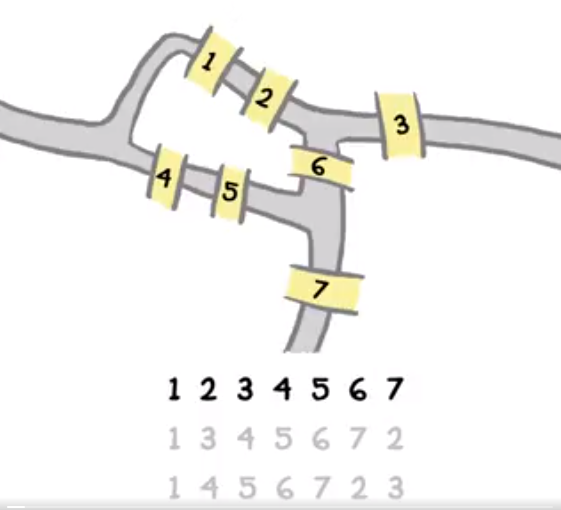
\includegraphics[width=.6\textwidth,height=.6\textheight]{../LectureF15/lecture5-fig1.png} }
   
%\date{ {\tiny Figure Source: \url{https://www.slideshare.net/Pokar/echelon-forms-45699354} } } 
\date{}

\begin{document}
\frame[plain]{\titlepage}

\begin{frame}[plain]{Trees}
  
  {\bf Definition 9.1.} A \Blue{tree} is a connected undirected graph with no simple circuits.
  \pause
  
  \medskip
  
  Because a tree cannot have a simple circuit, a tree \Red{cannot} contain multiple edges or loops.
   Therefore, any tree must be a simple graph. \pause
  \medskip
  
   {\bf Example 9.2.} Which of these graphs are trees?
     \begin{center}
        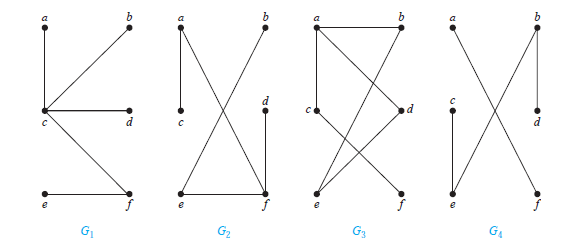
\includegraphics[height=3.5cm]{./img/lecture9-fig1.png}
      \end{center}
      \pause 
  
    {\bf Theorem 9.3.} An undirected graph is a tree 
    \Blue{if and only if} there is a \Red{unique simple
     path} between any two of its vertices.
     
\end{frame}

\begin{frame}[plain]{Forests}
  
    {\bf Definition 9.4.} A \Blue{forest} is a graph with no simple circuit
      but is not connected. Each of the connected components in a forest is a tree.
     \begin{center}
        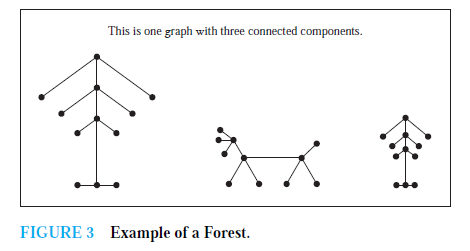
\includegraphics[height=4.5cm]{./img/lecture9-fig2.png}
      \end{center}

  
\end{frame}

\begin{frame}[plain]{}

{\bf Example 9.5.} Which of these are trees? Any forest?
 \begin{center}
        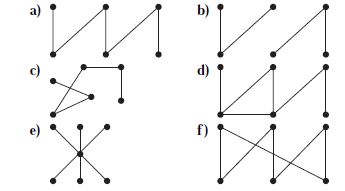
\includegraphics[height=5cm]{./img/lecture9-fig8.png}
      \end{center}
      
      
\end{frame}


\begin{frame}[plain]{Rooted Trees}
  
   {\bf Definition 9.6.} A \Blue{rooted tree} is a tree in which one vertex
      has been designated as the \Blue{root} and every edge is
	directed away from the root.
	
     \begin{center}
        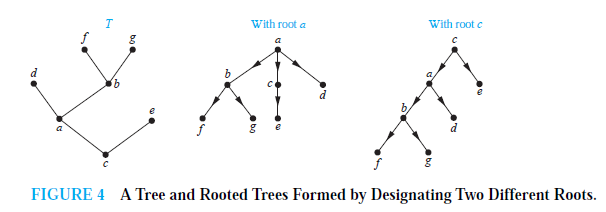
\includegraphics[height=4cm]{./img/lecture9-fig3.png}
      \end{center}
 
   An unrooted tree can be converted into different rooted
	trees when different vertices are chosen as the root. 
 
\end{frame}

\begin{frame}[plain]{Terminology for Rooted Trees~\footnote{
    Terminology for rooted trees is a mix of botany and
      genealogy (such as the family tree of the Bernoulli family of
      mathematicians).
      } }
      
 %    \begin{center}
 %       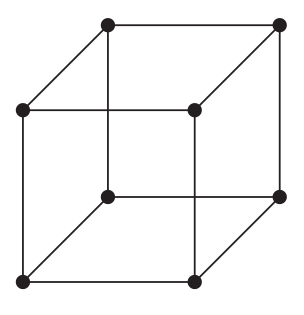
\includegraphics[height=5cm]{lecture8-fig4.png}
 %     \end{center}
 
   If $v$ is a vertex of a rooted tree other than the root, the \Blue{parent} of v is 
    the unique vertex $u$ such that there is a directed edge from $u$ to $v$. 
    \begin{center}
        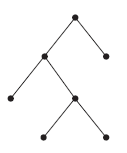
\includegraphics[height=3.5cm]{./img/lecture9-fig9.png}
      \end{center}
   \pause
   
    When $u$ is a parent of $v$, $v$ is called a \Blue{child} of u. Vertices with
    the same parent are called \Blue{siblings}.   
   
\end{frame}

\begin{frame}[plain]{ }
  
  The \Blue{ancestors} of a vertex are the vertices in the path from the root to this vertex, 
    excluding the vertex itself and including the root. 
    
    \begin{center}
        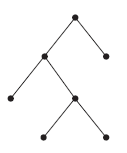
\includegraphics[height=3.5cm]{./img/lecture9-fig9.png}
      \end{center}
   \pause
   
   The \Blue{descendants} of a vertex $v$ are those vertices that have $v$ as
    an ancestor.
    
\end{frame}

\begin{frame}[plain]{ }
  
  A vertex of a rooted tree with no children is called a \Blue{leaf}. 
    Vertices that have children are called \Blue{internal vertices}.
    
    \begin{center}
        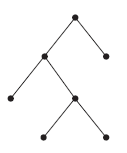
\includegraphics[height=3.5cm]{./img/lecture9-fig9.png}
      \end{center}
   \pause
   
    If $a$ is a vertex in a tree, the subtree with $a$ as its root is 
    the \Blue{subgraph of the tree} consisting of $a$
    and its descendants and all edges incident to these descendants.
    
\end{frame}

\begin{frame}[plain]{}

 \begin{center}
  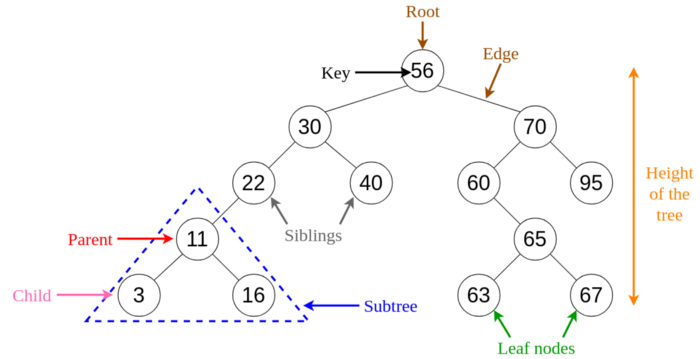
\includegraphics[height=6cm]{./img/lecture9-fig13.png}
 \end{center}
 
\end{frame}


%\begin{frame}[plain]{ }

%Summary:
%  \begin{itemize}
%    \item If $v$ is a vertex of a rooted tree other than the root, the \Blue{parent} of v is 
%    the unique vertex $u$ such that there is a directed edge from $u$ to $v$. 
%    \item When $u$ is a parent of $v$, $v$ is called a \Blue{child} of u. Vertices with
%    the same parent are called \Blue{siblings}.
%    \item The \Blue{ancestors} of a vertex are the vertices in the path from the root to this vertex, 
%    excluding the vertex itself and including the root. 
%    \item  The \Blue{descendants} of a vertex $v$ are those vertices that have $v$ as
%    an ancestor.
%    \item A vertex of a rooted tree with no children is called a \Blue{leaf}. 
%    Vertices that have children are called \Blue{internal vertices}.
%    \item  If $a$ is a vertex in a tree, the subtree with $a$ as its root is 
%    the \Blue{subgraph of the tree} consisting of $a$
%    and its descendants and all edges incident to these descendants.
%  \end{itemize}
%\end{frame}

\begin{frame}[plain]{}
  
    {\bf Practice 9.7.} In the rooted tree $T$ (with root $a$):
      \begin{enumerate}
       \item Find the parent of $c$, the children of $g$, the siblings
	  of $h$, the ancestors of $e$, and the descendants of $b$.
	\item Find all internal vertices and all leaves.
	\item  What is the subtree rooted at $g$?
      \end{enumerate}
      \begin{center}
        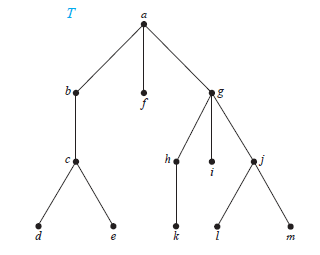
\includegraphics[height=5cm]{./img/lecture9-fig5.png}
      \end{center}

\end{frame}

\begin{frame}[plain]{$m$-ary Rooted Trees }
  
    {\bf Definition 9.8.} A rooted tree is called an \Blue{m-ary tree} if every internal vertex has no
      more than $m$ children. The tree is called a \Blue{full m-ary tree} if every internal
      vertex has exactly $m$ children. An $m$-ary tree with $m = 2$ is called a \Blue{binary tree}.
      \medskip
      
    {\bf Example 9.9.} Are the following rooted trees full $m$-ary trees for some positive
      integer $m$?
      \begin{center}
        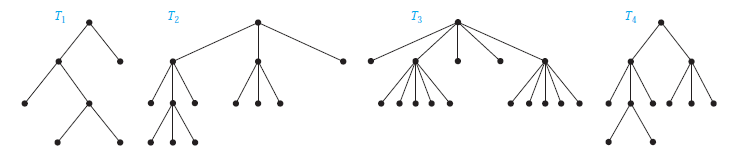
\includegraphics[height=3cm]{./img/lecture9-fig6.png}
      \end{center}

\end{frame}


\begin{frame}[plain]{Properties of Trees}
 
  {\bf Theorem 9.10.} A tree with $n$ vertices has $n-1$ edges. %(Proof by the mathematical induction)
  \pause
  \medskip
  
   {\bf Theorem 9.11.} A \Red{full $m$-ary tree} with $i$ internal vertices
      has \Blue{$n=m\times i+1$} vertices.
      \pause
      \medskip
      
 % {\bf Example 9.12.} How many vertices does a full 5-ary tree with 100 internal vertices have?
 % \pause
 % \medskip
  
  
  {\bf Theorem 9.12} Theorem 9.11 gives the following properties:
    \begin{enumerate}
     \item A \emph{full $m$-ary tree} {\bf with \Blue{$n$} vertices} has \Blue{$i=(n-1)/m$} internal vertices
	and \Blue{$\ell=[(m-1)n + 1]/m$} leaves,
      \item A \emph{full $m$-ary tree} {\bf with \Blue{$i$} internal vertices} has \Blue{$n=mi+1$} vertices and
	    \Blue{$\ell=(m-1)i+1$} leaves, 
      \item A \emph{full $m$-ary tree} {\bf with \Blue{$\ell$} leaves} has \Blue{$n=(m\ell-1)/(m-1)$} vertices and
	  \Blue{$i=(\ell-1)/(m-1)$} internal vertices.
    \end{enumerate}
    \pause
    
 {\bf Example 9.13.}  How many edges and leaves does a full binary tree 
      with 2000 internal vertices have?

\end{frame}

\begin{frame}[plain]{}

    \begin{enumerate}
     \item A \emph{full $m$-ary tree} {\bf with \Blue{$n$} vertices} has \Blue{$i=(n-1)/m$} internal vertices
	and \Blue{$\ell=[(m-1)n + 1]/m$} leaves,
      \item A \emph{full $m$-ary tree} {\bf with \Blue{$i$} internal vertices} has \Blue{$n=mi+1$} vertices and
	    \Blue{$\ell=(m-1)i+1$} leaves, 
      \item A \emph{full $m$-ary tree} {\bf with \Blue{$\ell$} leaves} has \Blue{$n=(m\ell-1)/(m-1)$} vertices and
	  \Blue{$i=(\ell-1)/(m-1)$} internal vertices.
    \end{enumerate}
\medskip

{\bf Practice 9.14.}
Suppose that someone starts a chain letter. Each person who receives the letter 
is asked to send
it on to four other people. Some people do this, but others do not send any letters. 
How many
people have seen the letter, including the first person, if no one receives more than one letter
and if the chain letter ends after there have been 100 people who read it
 but did not send it out?
How many people sent out the letter?
%Rosen, sec 11.1, p789, Ex 9
\vspace{0.3in}

\end{frame}

\begin{frame}[plain]{Depth and Height}

 The \Blue{depth} $d(v)$ of a node $v$ in a rooted tree is the number of edges
    in the path from the root to $v$. The \Blue{height} of a rooted tree is the maximum value of $d(v)$
    over all the nodes in the tree. 
    In other words, the height of a rooted tree
     is the length of the longest path from the root to any vertex.\pause

\begin{columns}[c]
   \column{.5\textwidth} 
     {\bf Example 9.15.} Find the depth of each vertex in the rooted tree shown below. 
 What is the height of this tree?
 \vspace{.5in}
 
   \column{.4\textwidth}
     \begin{center}
        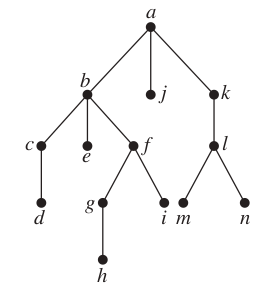
\includegraphics[height=3.5cm]{./img/lecture9-fig10.png} 
      \end{center}  
  \end{columns}
     \pause
 
 {\bf Theorem 9.16.} There are \Red{at most} \Blue{$m^h$} leaves in an $m$-ary tree of height $h$; 
 \Blue{$\ell \leq m^h$}.
 
\end{frame}

\begin{frame}[plain]{}

A rooted $m$-ary tree of height $h$ is \Blue{balanced} if all leaves are at depths $h$ or $h-1$.

\medskip

{\bf Example 9.17.} Which of the rooted trees are balanced?
\begin{center}
        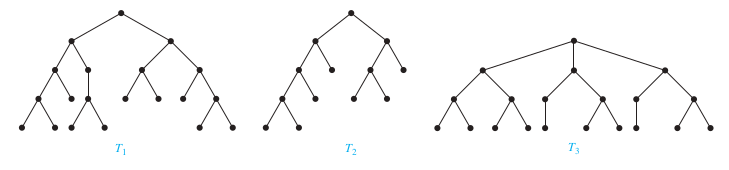
\includegraphics[height=3cm]{./img/lecture9-fig11.png}
      \end{center}
\pause

{\bf Corollary 9.18.} If an $m$-ary tree of height $h$ has $\ell$ leaves, then
 $\Blue{h \geq \lceil\log_m\ell\rceil}$.\\ 
 If the $m$-ary tree is full and balanced, then 
 $\Blue{h = \lceil\log_m\ell\rceil}$.
 %fulll and balanced or full and perfectly balanced?
\smallskip

{\small (We are using the ceiling function here. Recall that $\lceil x \rceil$
 is the smallest integer greater than or equal to $x$.)}
 
\end{frame}


\begin{frame}[plain]{}


{\bf Activity 9.19.} A full $m$-ary tree $T$ has 81 leaves and height 4.
    \begin{itemize}
     \item[(a)] Give the upper and lower bounds for $m$.
     \item[(b)] What is $m$ if $T$ is also balanced?
    \end{itemize}
 
\vspace{1.5in} 
 
\end{frame}

\end{document}

%%%%%%%%%%%%%%

\begin{frame}[plain]{Exercises}

  \begin{enumerate}
  % \setcounter{enumi}{7}
     \item Show that a full $m$-ary balanced tree of height $h$ has more than $m^{h-1}$ leaves.
  \item How many edges are there in a forest of $t$ trees containing a total of $n$ vertices?
  \item Either draw a full $m$-ary tree with 76 leaves and height 3,
    where $m$ is a positive integer, or show that no such tree exists.
    \medskip
    
   \item The \Blue{eccentricity} of a vertex in an unrooted tree is the length
	of the longest simple path beginning at this vertex. A vertex is
	called a \Blue{center} if no vertex in the tree has a smaller eccentricity
	than this vertex.
	\begin{columns}[c]
   \column{.35\textwidth} 
      Find every vertex that is a center in the given trees, $T1$ and $T2$. 
 \vspace{1.1in}
 
   \column{.42\textwidth}
     \begin{center}
        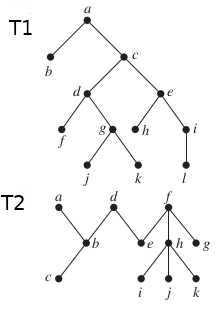
\includegraphics[height=5cm]{lecture9-fig12.png} 
      \end{center}  
  \end{columns}
  \end{enumerate}
  
\end{frame}


\begin{frame}{Ordered Rooted Trees }
  \begin{itemize}
    \item {\bf Definition} An \Blue{ordered rooted tree} is a rooted tree 
    where the children of each internal vertex are ordered.
       \item We draw ordered rooted trees so that the children of each internal vertex are shown in order
	  from left to right.
	  \begin{center}
        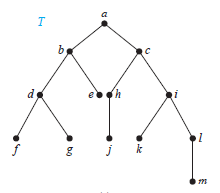
\includegraphics[height=3.5cm]{lecture9-fig7.png}
      \end{center}
      
  \end{itemize}
\end{frame}

\begin{frame}{Ordered Binary Trees }
  \begin{itemize}
    \item {\bf Definition} An \Blue{ordered binary tree} is an ordered rooted tree where each internal 
    vertex has at most two children. 
    \item If an internal vertex of a binary tree has two children, 
    the first is called the \Blue{left child} and
    the second the \Blue{right child}. 
    \item The tree rooted at the left child of a vertex is 
    called the \Blue{left subtree} of this vertex, and the tree rooted at the right child of 
    a vertex is called the \Blue{right subtree} of this vertex.
  \end{itemize}
\end{frame}

\begin{frame}{Ordered Rooted Trees }
  \begin{itemize}
    \item {\bf Example} Consider the binary tree $T$. \\
       (a) What are the left and right children of $d$? \\
	(b) What are the left and right subtrees of $c$?
      \begin{center}
        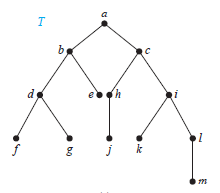
\includegraphics[height=3.5cm]{lecture9-fig7.png}
      \end{center}
  \end{itemize}
\end{frame}

